\documentclass[lettersize,journal]{IEEEtran}
\IEEEoverridecommandlockouts

\usepackage{cite}
\usepackage{amsmath,amssymb,amsfonts}
\usepackage{algorithmic}
\usepackage{graphicx}
\usepackage{textcomp}
\usepackage{xcolor}
\usepackage{subcaption}
\usepackage{url}
\usepackage{booktabs}
\usepackage{multirow}
\usepackage{makecell}
\usepackage[table]{xcolor}
\usepackage{array}
\usepackage{hhline}
\usepackage{comment}

\usepackage[top=0.75in, bottom=1in, left=0.625in, right=0.625in]{geometry}

% Sample-image tiles (same macro style as the authors' previous article)
\definecolor{cclean}{HTML}{4d4d4d}
\definecolor{chaze}{HTML}{7f7f7f}
\definecolor{cdehaze}{HTML}{2ca02c}
\definecolor{clow}{HTML}{1f1f1f}
\definecolor{cgamma}{HTML}{ff7f0e}
\newlength{\sampleimgw}
\newcommand{\smplimg}[2]{%
  {\setlength{\fboxsep}{0.8pt}\setlength{\fboxrule}{0.5pt}%
   \fcolorbox{#1}{white}{\includegraphics[width=\sampleimgw]{sample_images/#2}}}}

% ---------------------------------------------------------------
% DRAFT NOTES (red) mark text that still waits for the real-data runs
% (RRSHID real haze, CODrone real night) or for a final check.
% Set \drafttrue to \draftfalse to hide them before submission.
\newif\ifdraft \draftfalse
\newcommand{\draftnote}[1]{\ifdraft{\color{red}\footnotesize[#1]}\fi}
% ---------------------------------------------------------------

\def\BibTeX{{\rm B\kern-.05em{\sc i\kern-.025em b}\kern-.08em
    T\kern-.1667em\lower.7ex\hbox{E}\kern-.125emX}}

\begin{document}

\title{Detect, Then Enhance: Lightweight Degradation-Aware Enhancement Routing for Frozen Remote-Sensing Vision-Language Models}

\author{Syed Muhammad Hamza Tauqeer, Muhammad Talha, Huma Ghafoor*, and Seung Yeob Nam*,
\IEEEmembership{Senior Member, IEEE}
\thanks{S.M.H. Tauqeer is with the Military College of Signals (MCS), National University of Sciences and Technology (NUST), Islamabad, 44000, Pakistan (e-mail: stauqeer.msee24mcs@student.nust.edu.pk)}
\thanks{M. Talha and H. Ghafoor are with the School of Electrical Engineering and Computer Science (SEECS), National University of Sciences and Technology (NUST), Islamabad, 44000, Pakistan (e-mail: (muhtalha.bee20seecs, huma.ghafoor)@seecs.edu.pk)}
\thanks{Prof. Nam is with the Department of Information and Communication Engineering, Yeungnam University,
280 Daehak-Ro, Gyeongsan, Gyeongbuk 38541, South Korea (e-mail: synam@ynu.ac.kr)}
\thanks{*Correspondence: H. Ghafoor and S. Y. Nam}}

\markboth{IEEE Journal of Selected Topics in Applied Earth Observations and Remote Sensing}%
{Tauqeer \MakeLowercase{\textit{et al.}}: Detect, Then Enhance: Degradation-Aware Enhancement Routing for RS-VLMs}
\maketitle

\begin{abstract}
Vision-language models (VLMs) are increasingly used to answer questions about remote-sensing images, yet operational imagery is often hazy or underexposed, and a common response is to enhance every image before inference. We measure how classical enhancement changes the answers of frozen VLMs and propose a lightweight router that selects the enhancement per image without fine-tuning or querying the VLM. Two frozen models, Qwen2.5-VL-3B and Qwen2-VL-2B, answer scene, surface, and object questions about 700 UC Merced images under clean, hazy, and low-light conditions at three severities, with each input passed through no enhancement, CLAHE, adaptive gamma correction, or dark-channel dehazing (27,300 scored runs per model). Blind enhancement is unreliable: CLAHE lowers clean-image accuracy by 3.1 and 2.8 points for the two models, dehazing does not help low-light inputs, and each degradation has a different best operator. The router identifies the degradation from 11 global image statistics (94.7\% accuracy) and applies the operator that works best for it. It raises accuracy from 79.6\% to 83.3\% for Qwen2.5-VL-3B and from 85.2\% to 86.2\% for Qwen2-VL-2B, matches an oracle that knows the true degradation, and outperforms the best fixed operator for both models. Fitted once on UC Merced and applied unchanged, the router transfers to the AID dataset (+2.5 and +0.9 points) and to a stronger, unseen degradation level (+8.9 and +3.6 points). On real hazy satellite images from RRSHID, dehazing remains the right operator, but a detector built only on synthetic haze misses part of the real haze; adding 30 labelled real image pairs to the detector, without touching the VLM or the lookup table, raises detection to 98--99\% and brings the router to oracle accuracy on hazy inputs. On real night-time UAV images from CODrone, no operator changed accuracy by more than 2 points, so routing matters little there. Code and all scored runs are publicly available.
\end{abstract}

\begin{IEEEkeywords}
Dehazing, image enhancement, low-light enhancement, remote sensing, robustness, test-time preprocessing, vision-language models (VLMs), visual question answering (VQA).
\end{IEEEkeywords}


\section{Introduction}

Vision-language models (VLMs) have changed how users interact with Earth-observation data: instead of training a task-specific network, a user can ask a question about an image in natural language and receive an answer~\cite{li2024vlmrs, weng2025vlmrs}. Remote-sensing visual question answering (RSVQA) formalised this idea~\cite{lobry2020rsvqa}, and instruction-tuned models such as GeoChat~\cite{kuckreja2024geochat}, EarthGPT~\cite{zhang2024earthgpt}, and LHRS-Bot~\cite{muhtar2024lhrsbot} extend general multimodal models to remote-sensing dialogue. General-purpose VLMs such as Qwen2-VL~\cite{wang2024qwen2vl} and Qwen2.5-VL~\cite{bai2025qwen25vl} are also applied to such imagery directly, without domain fine-tuning. In operational settings, however, images are rarely as clean as benchmark data: haze reduces contrast and shifts colour, and low sun angles or underexposure darken scenes and raise relative noise.

Recent work on this problem has advanced along three lines. The first measures how much corruptions hurt. For general multimodal models, MLLM-IC covers 40 corruption types~\cite{qiu2025mllmic}, R-Bench pairs real-world corrupted images with their references~\cite{li2024rbench}, and VLM-RobustBench studies how corruption type and severity affect VLM answers~\cite{saxena2026vlmrobustbench}. For Earth observation, REOBench evaluates foundation models across six tasks and twelve corruption types, including haze, and reports accuracy drops ranging from less than 1\% to over 25\%~\cite{li2025reobench}, and SenseBench asks whether VLMs can perceive and describe remote-sensing degradations themselves~\cite{zhong2026sensebench}. The second retrains models to resist corruptions: RemoteShield trains a remote-sensing multimodal model with preference learning over clean and perturbed inputs~\cite{min2026remoteshield}. Retraining, however, must be repeated for each model and is out of reach for most users of off-the-shelf VLMs. The third line restores the input before the downstream model sees it. Remote-sensing dehazing alone has produced more than a hundred methods~\cite{zhou2026rsdehazing}, and plug-and-play enhancement branches have been attached to aerial object detectors so that hazy inputs can be handled without retraining the detector~\cite{wu2024plugplay}. Yet better-looking images do not reliably give better machine predictions. Kumar and Chadha~\cite{kumar2025fogfailure} showed that dehazing can harm object detection on clear images, and a recent benchmark of defogging pipelines found that gains in image fidelity do not consistently carry over to detection and segmentation~\cite{aryashad2025filters}. For multimodal large language models, Xing~et~al.~\cite{xing2025vqparadox} reported a visual-quality paradox: performance can improve when images deviate from human-perceived fidelity.

Several methods therefore choose the restoration per input. DA-CLIP adapts a pretrained vision-language model to predict degradation-aware embeddings that steer a restoration network~\cite{luo2024daclip}, and Cai~et~al.~\cite{cai2025degradationaware} use Qwen2.5-VL to classify the degradation type of an image and then call a matching restoration model. Both judge success by restored image quality rather than by the answers of a downstream VLM. For multimodal models, CARES trains a module that predicts the minimal sufficient input resolution for each image--question pair~\cite{kimhi2025cares}, DocIntent lets a multimodal model invoke restoration tools on document images and roll back unhelpful edits~\cite{huang2026docintent}, and V-QPP-Bench shows that off-the-shelf multimodal models struggle to select preprocessing tools without specialised training~\cite{zeng2026fixbeforesearch}. These methods target other domains, select a resolution rather than an enhancement, or place a large model in the loop, which adds model calls for every input.

Three limitations recur. First, preprocessing for remote-sensing VLMs is usually applied blindly or not at all, and its effect on answer accuracy, rather than on image-quality metrics, is rarely measured. Second, it is unclear whether a frozen VLM can recover accuracy through cheap per-image operator selection, and whether such a selector, once built, still works on another dataset, another VLM, a degradation stronger than any seen during its construction, or real rather than synthetic degradations. Third, a preprocessing gain is only meaningful when the answers depend on the image, which is not guaranteed for remote-sensing VQA benchmarks, as the RSVQA-LR pilot in Section~\ref{sec:pilot} shows.

This work addresses these gaps with a controlled study and a simple router. Questions about UC Merced images~\cite{yang2010ucm, chaudhuri2018multilabel} are posed to two frozen VLMs under clean, hazy, and low-light conditions at three severities, and each input is passed through one of four operators: none, contrast-limited adaptive histogram equalisation (CLAHE), adaptive gamma correction, or dark-channel dehazing. Every question is also asked with a blank grey image to measure how much the answer depends on the picture. The router first detects the degradation from 11 global image statistics and then applies the operator that performed best for that degradation on training questions; it never calls the VLM. The router built on UC Merced is then applied, without any change, to the AID dataset~\cite{xia2017aid}, to an unseen, stronger degradation level, to real hazy satellite images from RRSHID~\cite{zhu2025rrshid}, and to real night-time UAV images from CODrone~\cite{ye2025codrone}.

The main contributions are as follows:

\begin{enumerate}
    \item \textbf{Controlled measurement of enhancement effects on two frozen VLMs:} Three input conditions at three severities are crossed with four classical operators and three question types, so the benefit and harm of each operator are measured on answer accuracy rather than on image-quality metrics.

    \item \textbf{Lightweight degradation-aware router:} A classifier on 11 global statistics identifies the degradation with 94.7\% accuracy, and a lookup table selects the operator. The router needs no VLM fine-tuning, adds no VLM calls, and costs 15--28\,ms of CPU time per image. On synthetic degradations, a two-threshold version of the detector performs almost as well.

    \item \textbf{Transfer to new data and real degradations:} The router fitted on UC Merced is applied unchanged to AID, to a stronger unseen degradation level, and to the other VLM, and keeps its gain in each case. On real haze, the detector is the only component that needs adapting: 30 labelled real image pairs bring the router to oracle accuracy on hazy inputs. On real night imagery, enhancement itself changes accuracy by less than 2 points.

    \item \textbf{Generation-free scoring protocol:} Each answer is read from the first-token probabilities of a single forward pass, removing answer-parsing errors and keeping the full study within two free-tier T4 GPUs.

    \item \textbf{Blank-image control for benchmark validity:} On RSVQA-LR, accuracy with a grey image (67.3\%) matches accuracy with the real image (67.0\%), so preprocessing effects measured there are not interpretable for the tested subset and model.
\end{enumerate}


\section{Methodology}

\subsection{Overview of the Proposed Experimental Framework}

This study contributes an evaluation protocol and a lightweight routing rule rather than a new network. The protocol measures how classical enhancement changes the answers of a frozen VLM on remote-sensing questions under controlled degradations. Every experimental factor is held fixed across conditions, including the question set, the prompt template, the degradation parameters, the enhancement settings, and the scoring rule, so that differences in accuracy can be attributed to the input condition and the enhancement operator alone. The pipeline, shown in Fig.~\ref{fig:pipeline}, covers question construction, degradation synthesis, enhancement, generation-free VLM scoring, and the offline construction of the router. The VLMs are never fine-tuned, and the router never queries them.

\begin{figure*}[t]
    \centering
    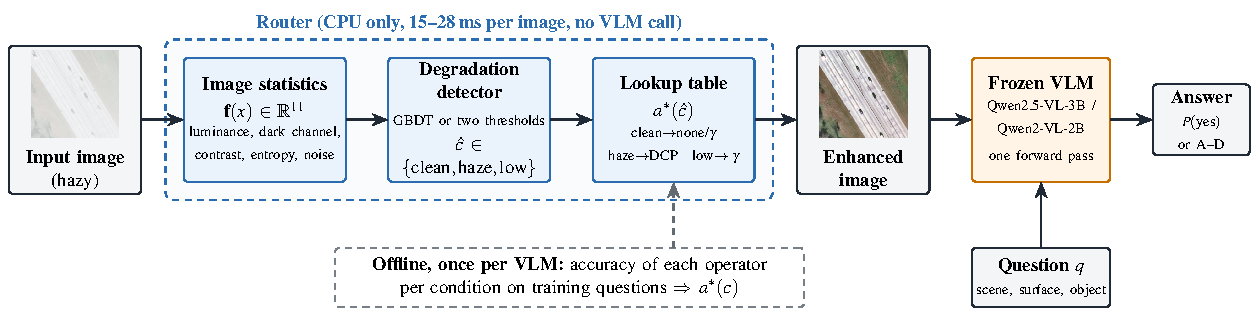
\includegraphics[width=0.9\textwidth]{Flowchart.pdf}
    \caption{Proposed degradation-aware enhancement routing. Global statistics of the input image are mapped to a degradation class, a lookup table selects the enhancement operator, and the frozen VLM answers from the enhanced image. The lookup table is built offline from cross-validated accuracies; no VLM call is made at routing time.}
    \label{fig:pipeline}
\end{figure*}

\subsection{Dataset Sources and Question Construction}

The main study uses the UC Merced land-use dataset~\cite{yang2010ucm}, which contains 2,100 aerial images of 256$\times$256 pixels at about 0.3\,m resolution, 100 for each of 21 scene classes. Its multi-label release~\cite{chaudhuri2018multilabel} annotates every image with one or more of 17 object and surface labels. These two label sets allow three question types on the same image. \emph{Scene} questions ask for the land-use class among four options, with three distractors drawn at random from the other classes and the correct letter balanced across A--D. \emph{Surface} questions ask whether water, sea, sand, grass, trees, a crop field, chaparral, bare soil, or pavement is present. \emph{Object} questions ask whether an airplane, building, car, sports court, dock, mobile home, ship, or storage tank is present. Surface answers are balanced, whereas about one third of object answers are \emph{yes}, because many scenes contain none of the eight objects. Scene questions rely on overall layout and texture, surface questions on colour and extent, and object questions on small, edge-defined details. The main study samples 700 images and three questions per image.

The cross-dataset test uses AID~\cite{xia2017aid}, which contains 10,000 aerial images of 600$\times$600 pixels in 30 scene classes collected from Google Earth. Scene questions are built from 20 images per class (600 images), and surface and object questions from 400 images of the AID multi-label release, which uses the same 17 labels as UC Merced; all AID images are resized to 512$\times$512 pixels. The unseen-severity test uses 200 further UC Merced images that do not appear in the main study.

Two further sets contain real degradations. RRSHID~\cite{zhu2025rrshid} provides real hazy satellite images, each paired with a haze-free image of the same scene, in thin, moderate, and thick haze subsets. From its test split, 50 pairs per density were drawn (150 pairs), resized to 512$\times$512 pixels, and each image received five presence questions (buildings, trees, water, a road, farmland). RRSHID has no question labels, so the reference answer for each question is the VLM's own answer on the haze-free twin, kept only when the model is confident ($P(\text{yes}) > 0.8$ or $< 0.2$); accuracy on RRSHID therefore measures agreement with the haze-free answer. CODrone~\cite{ye2025codrone} provides UAV images of 3840$\times$2160 pixels captured by day and at night, with oriented-box labels for 12 object categories; its file names state whether an image was taken by day or at night. From its test split, 150 night and 100 day images were drawn, resized to at most 768 pixels on the long side, and each received four presence questions about the 12 object classes (the \emph{ignored} mask label was excluded), half with a \emph{yes} answer where possible, answered from the box labels.

Two pilot studies preceded the main study. The first used 300 yes/no presence and comparison questions on 100 images of the RSVQA low-resolution (LR) test split~\cite{lobry2020rsvqa}, built from Sentinel-2 tiles and OpenStreetMap labels. The second used 300 four-option scene questions on 300 UC Merced images. Table~\ref{tab:data} summarises all studies.

\begin{table}[t]
\centering
\footnotesize
\caption{Datasets and questions used in each study.}
\label{tab:data}
\setlength{\tabcolsep}{2.5pt}
\resizebox{\linewidth}{!}{
\begin{tabular}{|l|c|c|l|}
\hline
\textbf{Study} & \textbf{Images} & \textbf{Questions} & \textbf{Conditions} \\
\hline
Pilot 1: RSVQA-LR~\cite{lobry2020rsvqa} & 100 & 300 & Synthetic, severity 1--3 \\
Pilot 2: UC Merced~\cite{yang2010ucm} & 300 & 300 & Synthetic, severity 1--3 \\
Main: UC Merced multi-label~\cite{chaudhuri2018multilabel} & 700 & 2,100 & Synthetic, severity 1--3 \\
\hline
Transfer: AID~\cite{xia2017aid} & 1,000 & 1,400 & Synthetic, severity 1--3 \\
Transfer: unseen severity (UC Merced) & 200 & 600 & Synthetic, severity 4 \\
Transfer: RRSHID~\cite{zhu2025rrshid} & 150 pairs & 750 & Real haze (thin, moderate, thick) \\
Transfer: CODrone~\cite{ye2025codrone} & 250 & 1,000 & Real night (150) and day (100) \\
\hline
\end{tabular}}
\caption*{\footnotesize In the synthetic studies each question is answered under 3 conditions $\times$ 4 operators plus one blank-image control (13 runs per question; 27,300 runs per VLM in the main study). RRSHID questions are answered on the hazy image and its haze-free twin, and CODrone questions on the night or day image, each with the 4 operators plus the blank control.}
\end{table}

\subsection{Degradation Model and Severity Levels}

Haze is synthesised with the atmospheric scattering model~\cite{narasimhan2002vision}. For a clean image $J$ with intensities in $[0,1]$, the hazy image at pixel $p$ is
\begin{equation}
I(p) = J(p)\,t(p) + A\,\big(1 - t(p)\big),
\label{eq:haze}
\end{equation}
where $A \sim \mathcal{U}(0.80, 0.95)$ is the airlight and $t(p)$ is a transmission map formed by a base value $t_0$ plus a gentle linear ramp across the tile (slope drawn from $\mathcal{U}(-0.1, 0.1)$ in each direction), clipped to $[0.15, 0.95]$ so that haze density varies smoothly across the scene. Low light combines a gamma curve, a global gain, and additive sensor noise:
\begin{equation}
I(p) = s\,J(p)^{\gamma} + n(p), \qquad n(p) \sim \mathcal{N}(0, \sigma^{2}).
\label{eq:lowlight}
\end{equation}
Low-light conditions are under-represented in common vision benchmarks~\cite{loh2019exdark}, which motivates their inclusion alongside haze. Each degraded image in the main and AID studies receives one of three severities, drawn uniformly per image and condition, with the parameter ranges in Table~\ref{tab:severity}. A fourth level is used only for the unseen-severity test: it has denser haze with a slightly coloured airlight (each channel of $A$ shifted by up to $\pm0.08$) and darker, noisier low light, and none of its images are used to build the router. All random draws are seeded by a hash of the image identifier and condition, so every image version can be regenerated exactly. Fig.~\ref{fig:samples} shows three images from the main study under both degradations, before and after the operator selected by the router, together with the answers of Qwen2.5-VL-3B.

\begin{table}[t]
\centering
\footnotesize
\caption{Degradation parameters at each severity level. Level 4 is used only for the unseen-severity test.}
\label{tab:severity}
\setlength{\tabcolsep}{3pt}
\begin{tabular}{|l|c|c|c|c|}
\hline
\textbf{Severity} & \textbf{Haze $t_0$} & \textbf{Low light $\gamma$} & \textbf{Gain $s$} & \textbf{Noise $\sigma$} \\
\hline
1 (mild)   & 0.60--0.75 & 1.4--1.8 & 0.55--0.70 & 0.008 \\
2 (medium) & 0.40--0.55 & 1.8--2.4 & 0.35--0.50 & 0.012 \\
3 (strong) & 0.20--0.35 & 2.4--3.0 & 0.20--0.30 & 0.018 \\
\hline
4 (unseen) & 0.08--0.18\textsuperscript{a} & 2.6--3.4 & 0.12--0.22 & 0.030 \\
\hline
\multicolumn{5}{|l|}{\footnotesize \textsuperscript{a}With a coloured airlight, each channel shifted by up to $\pm0.08$.} \\
\hline
\end{tabular}
\end{table}

\begin{figure*}[t]
\centering
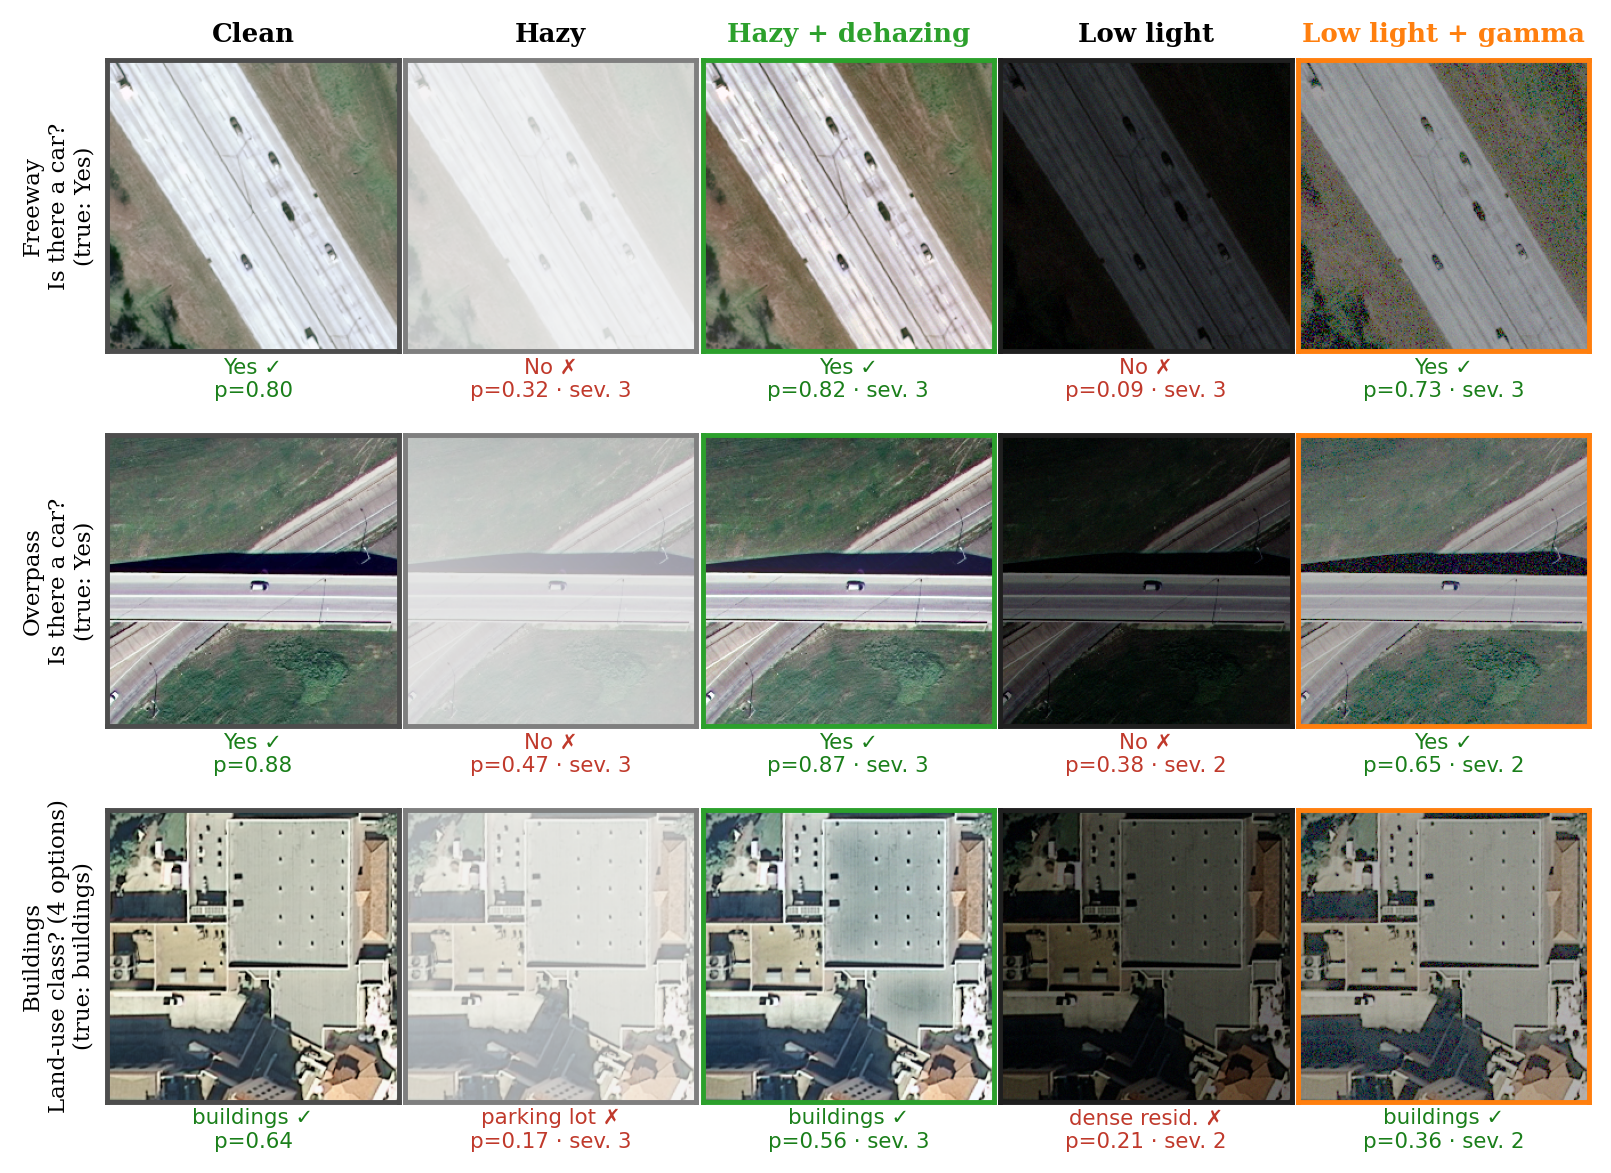
\includegraphics[width=0.95\textwidth]{graphs/qual_examples}
\caption{Examples from the main study, shown exactly as Qwen2.5-VL-3B received them. Each row is one question; the columns show the clean image, the hazy input and its dehazed version, and the low-light input and its gamma-corrected version, with the severity drawn in the experiment. Below each image are the model's answer (\checkmark\ correct, $\times$ wrong) and the probability it assigned to the correct answer. The examples were selected as cases in which the operator chosen by the router corrected a wrong answer under both degradations; they illustrate the mechanism and are not a random sample.}
\label{fig:samples}
\end{figure*}

\subsection{Enhancement Operators}

Four operators form the action set $\mathcal{E} = \{e_{\text{none}}, e_{\text{clahe}}, e_{\gamma}, e_{\text{dcp}}\}$; all are classical and need no training. CLAHE~\cite{zuiderveld1994clahe} is applied to the L channel of the CIELAB colour space with a clip limit of 2.0 and 8$\times$8 tiles. Adaptive gamma correction maps the mean luminance $\bar{L}$ of the input to 0.5:
\begin{equation}
e_{\gamma}(I) = I^{\,g}, \qquad g = \operatorname{clip}\!\left(\frac{\log 0.5}{\log \bar{L}},\, 0.3,\, 3.0\right),
\label{eq:gamma}
\end{equation}
so that it brightens dark images, darkens washed-out ones, and leaves well-exposed images almost unchanged. Dehazing uses the dark-channel prior~\cite{he2011dcp} with 15$\times$15 patches, $\omega = 0.95$, and a lower transmission bound of 0.1. The transmission is estimated on a copy of the image downscaled to at most 256 pixels on the long side, the airlight is taken per channel from the brightest 0.1\% of dark-channel pixels, and the transmission is refined with a guided filter~\cite{he2013guided} (grey-level guide, 30$\times$30 box window, $\varepsilon = 10^{-3}$) and upsampled before the scene radiance is recovered by inverting~\eqref{eq:haze}.

\subsection{Degradation-Aware Router}

The router chooses one operator per image without seeing the question or calling the VLM. In the first stage, 11 global statistics are computed from the input: luminance mean and standard deviation, RMS contrast, 64-bin luminance entropy, mean dark channel over 15$\times$15 patches, saturation mean and standard deviation, Laplacian variance, a median-absolute-deviation noise estimate, and the fractions of very dark ($<0.1$) and very bright ($>0.9$) pixels. A gradient-boosted tree classifier with 200 iterations~\cite{pedregosa2011sklearn} maps this vector $\mathbf{f}(x)$ to a condition $\hat{c} \in \{\text{clean}, \text{haze}, \text{low light}\}$. In the second stage, the router applies the operator that achieved the highest VLM accuracy for that condition on the training questions:
\begin{equation}
\pi(x) = a^{*}\big(\hat{c}(\mathbf{f}(x))\big), \qquad
a^{*}(c) = \arg\max_{e \in \mathcal{E}}\; \mathrm{Acc}_{\text{train}}(e \mid c).
\label{eq:router}
\end{equation}
A simpler detector uses only two of the statistics, the mean luminance $\bar{L}$ and the mean dark channel $\bar{D}$:
\begin{equation}
\hat{c}(x) =
\begin{cases}
\text{low light}, & \bar{L} < \theta_L,\\
\text{haze}, & \bar{L} \geq \theta_L \text{ and } \bar{D} > \theta_D,\\
\text{clean}, & \text{otherwise},
\end{cases}
\label{eq:threshold}
\end{equation}
where $\theta_L$ and $\theta_D$ are chosen by grid search to maximise detection accuracy on the training images. A further variant conditions the lookup on the question type, giving $a^{*}(c, \tau)$ for type $\tau$. The detector is independent of the VLM; only the lookup table depends on which VLM is being served.

\subsection{Per-Sample Gating Baseline}

To test whether a finer, per-image decision helps, a per-sample gate was also built. A gradient-boosted regressor predicts the VLM's probability of a correct answer for each (input, operator) pair from the 11 statistics, three measures of how much the operator changes the image (mean CIELAB $\Delta E$, mean hue shift in saturated pixels, and the ratio of high-frequency energy after and before), the operator identity, and the question type. The gate applies the operator with the highest predicted score only if it exceeds the score of $e_{\text{none}}$ by a margin of 0.02; otherwise it leaves the image unchanged.

\subsection{Generation-Free Answer Scoring}

Each run is a single forward pass with no text generation. For a yes/no question, let $\ell_w$ be the log-probability of token $w$ at the first answer position. The probability of a \emph{yes} answer is
\begin{equation}
P(\text{yes}) = \sigma\!\Big(\log\!\sum_{w \in \mathcal{Y}} e^{\ell_w} - \log\!\sum_{w \in \mathcal{N}} e^{\ell_w}\Big),
\label{eq:yesno}
\end{equation}
with $\mathcal{Y} = \{\text{Yes}, \text{yes}\}$, $\mathcal{N} = \{\text{No}, \text{no}\}$, and $\sigma$ the logistic function. For a four-option question, a softmax over the logits of the letter tokens A--D gives option probabilities, and the predicted answer is the arg-max. The prompt appends ``Answer with Yes or No.'' or ``Answer with only the letter of the correct option.'' to the question. For both VLMs, more than 99.8\% of the next-token probability mass fell on these answer tokens on average, so the restriction discards almost no probability. This protocol removes answer-parsing errors and yields a soft score, the probability assigned to the correct answer, alongside hard accuracy.

\subsection{Hardware and Inference Environment}

All VLM runs used Kaggle notebooks with two NVIDIA Tesla T4 GPUs (16\,GB each), Python 3.13, PyTorch 2.11 with CUDA 13.0, and Hugging Face Transformers 4.57~\cite{wolf2020transformers}. The questions were split into two shards, one per GPU, and each GPU held a full copy of the model. Qwen2.5-VL-3B-Instruct~\cite{bai2025qwen25vl} and Qwen2-VL-2B-Instruct~\cite{wang2024qwen2vl} ran in bfloat16 with scaled-dot-product attention, a batch size of 16, and at most 512$\times$512 input pixels. On 256$\times$256 UC Merced images, a run took about 0.6\,s per GPU for Qwen2.5-VL-3B and 0.4\,s for Qwen2-VL-2B; on 512$\times$512 AID and RRSHID images and on CODrone images with a 768-pixel long side, about 2.0--2.2\,s and 1.5--1.7\,s. The CODrone runs used Transformers 5.20, the platform default at the time, with the same model weights, prompts, and scoring; all other runs used 4.57. Degradations, enhancements, and image statistics were computed once per image version and cached.

\subsection{Reproducibility, Code Availability, and Result Storage}

Every image version is stored with its file name, condition, severity, operator, input statistics, and enhancement-drift measures, and every VLM run is stored as one record keyed by question, condition, and operator with the predicted answer, answer-token probabilities, and correctness. Runs are resumable, so an interrupted session continues from the last completed batch, and the GPU model, numerical precision, and library versions of each run are saved alongside the results. All random choices are seeded: question sampling and dataset preparation use seed 0, each degraded image version is generated from a seed derived from the image identifier and condition, so every version can be regenerated exactly, and the gradient-boosted models and the bootstrap use seed 0. Scoring involves no sampling, so a VLM answer is fixed once the software versions are fixed. The repository~\cite{detectthenenhance2026code} contains the code for every step, one script per experiment, a configuration file listing all settings above, the fitted router (detectors, thresholds, and lookup tables), the logs of the original runs, and every scored VLM run behind the tables, so all tables can be recomputed on a CPU without the images or the VLMs. Recomputing them with a different scikit-learn version than the one on Kaggle changed detector accuracies by at most about one point and router accuracies by at most 0.2 points.

\subsection{Evaluation Metrics}

Performance is measured by answer accuracy, the fraction of questions whose predicted answer matches the ground truth. To describe how an operator changes individual answers, the help rate and hurt rate of operator $e$ under condition $c$ are measured against no enhancement:
\begin{equation}
\text{Help}(e,c) = \frac{1}{N}\sum_{i=1}^{N}\mathbf{1}\big[\hat{y}^{\,e}_{i} = y_i \,\wedge\, \hat{y}^{\,\text{none}}_{i} \neq y_i\big],
\label{eq:help}
\end{equation}
with the hurt rate defined symmetrically for answers that turn from correct to wrong. In the main study, all learned policies are evaluated with 5-fold cross-validation grouped by image, so no image appears in both a training and a test fold. In the transfer studies, the detector, the thresholds, and the lookup table are fitted once on all main-study images and applied to the target data without any change. For RRSHID, a few-shot variant is also reported: the image statistics of $k$ labelled hazy/haze-free pairs per density from the RRSHID \emph{training} split are added to the detector's training data, while the VLM, the lookup table, and the test pairs stay unchanged. Differences between policies are reported with 95\% confidence intervals from a paired bootstrap~\cite{efron1993bootstrap} with 2,000 resamples:
\begin{equation}
\Delta = \frac{1}{U}\sum_{u=1}^{U}\big(\mathbf{1}[\hat{y}^{\,\pi_1}_u = y_u] - \mathbf{1}[\hat{y}^{\,\pi_2}_u = y_u]\big),
\label{eq:delta}
\end{equation}
where $U$ is the number of (question, condition) units and $\pi_1$, $\pi_2$ are the two policies compared. Gains over never enhancing in the main study resample units. Because the three questions of an image are not independent, comparisons between the router and the best fixed operator, and all transfer results, resample whole images instead, which gives wider and more conservative intervals. Finally, the blank-image control is the accuracy obtained when the image is replaced by a uniform grey image of the same size; it measures how much of the accuracy comes from the question text alone.


\section{Performance Evaluation}

\begin{figure*}[t]
\centering
\begin{subfigure}[t]{0.31\linewidth}
  \centering
  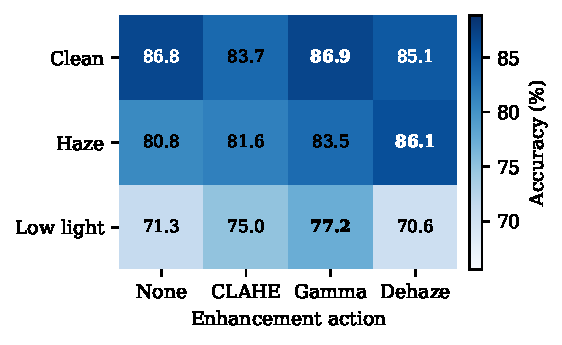
\includegraphics[width=\linewidth]{graphs/heatmap_cond_action}
  \caption{Accuracy by condition and operator.}
\end{subfigure}
\hfill
\begin{subfigure}[t]{0.31\linewidth}
  \centering
  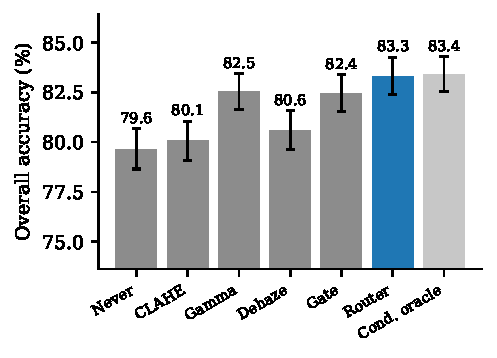
\includegraphics[width=\linewidth]{graphs/policy_accuracy}
  \caption{Overall accuracy of each policy.}
\end{subfigure}
\hfill
\begin{subfigure}[t]{0.31\linewidth}
  \centering
  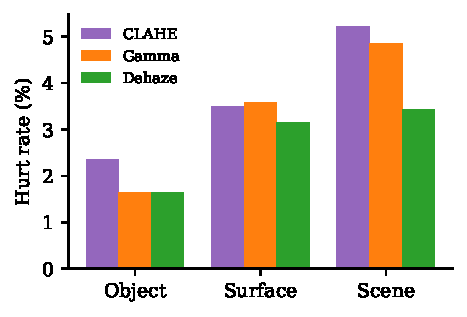
\includegraphics[width=\linewidth]{graphs/hurt_by_qtype}
  \caption{Hurt rate by question type.}
\end{subfigure}

\vspace{8pt}

\makebox[\linewidth][c]{%
\begin{subfigure}[t]{0.31\linewidth}
  \centering
  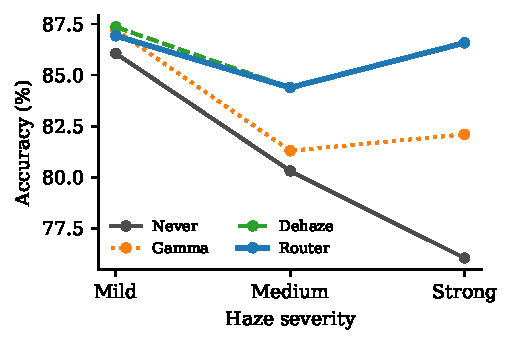
\includegraphics[width=\linewidth]{graphs/severity_haze}
  \caption{Accuracy versus haze severity.}
\end{subfigure}
\hspace{0.03\linewidth}
\begin{subfigure}[t]{0.31\linewidth}
  \centering
  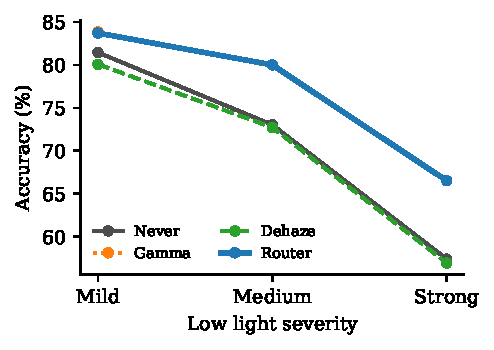
\includegraphics[width=\linewidth]{graphs/severity_lowlight}
  \caption{Accuracy versus low-light severity.}
\end{subfigure}
}

\caption{Summary of enhancement effects for Qwen2.5-VL-3B on the main study.
(a)~Accuracy for each input condition and enhancement operator; bold marks the best operator per condition.
(b)~Overall accuracy of fixed, learned, and oracle policies, with 95\% bootstrap confidence intervals.
(c)~Share of degraded inputs on which an operator turns a correct answer wrong, by question type.
(d)--(e)~Accuracy at each degradation severity for no enhancement, always-gamma, always-dehaze, and the router.}
\label{fig:results_summary}
\end{figure*}

Fig.~\ref{fig:results_summary} gives a visual summary of the main study for Qwen2.5-VL-3B, and Table~\ref{tab:main} reports the full numerical results for both VLMs. The sections below cover the pilot findings, the effect of each operator, the comparison of routing policies, the role of severity and question type, transfer to new data and a new degradation level, the source of harmful enhancements, computational cost, and a comparison with prior work.

\begin{table*}[!t]
\centering
\footnotesize
\caption{Accuracy (\%) of all policies on the main study (700 UC Merced images, 2,100 questions under each condition). Gain is measured against never enhancing, with 95\% paired-bootstrap confidence intervals. Learned policies use 5-fold cross-validation grouped by image.}
\label{tab:main}
\renewcommand{\arraystretch}{1.05}
\setlength{\tabcolsep}{3.5pt}
\resizebox{\linewidth}{!}{
\begin{tabular}{|l|c|c|c|c|c|c|c|c|c|c|}
\hline
 & \multicolumn{5}{c|}{\textbf{Qwen2.5-VL-3B}} & \multicolumn{5}{c|}{\textbf{Qwen2-VL-2B}} \\
\hline
\textbf{Policy} & \textbf{Clean} & \textbf{Haze} & \textbf{Low light} & \textbf{Overall} & \textbf{Gain [95\% CI]} & \textbf{Clean} & \textbf{Haze} & \textbf{Low light} & \textbf{Overall} & \textbf{Gain [95\% CI]} \\
\hline
Never enhance & 86.8 & 80.8 & 71.3 & 79.6 & -- & \textbf{88.6} & 85.2 & 81.8 & 85.2 & -- \\
Always CLAHE & 83.7 & 81.6 & 75.0 & 80.1 & +0.5 [$-$0.4, +1.2] & 85.8 & 84.3 & 80.5 & 83.5 & $-$1.7 [$-$2.3, $-$1.0] \\
Always gamma & \textbf{86.9} & 83.5 & \textbf{77.2} & 82.5 & +2.9 [+2.2, +3.7] & 87.5 & 86.8 & \textbf{82.5} & 85.6 & +0.4 [$-$0.2, +1.0] \\
Always dehaze & 85.1 & \textbf{86.1} & 70.6 & 80.6 & +1.0 [+0.3, +1.7] & 87.1 & \textbf{87.5} & 81.8 & 85.5 & +0.3 [$-$0.3, +0.9] \\
\hline
Per-sample gate & \textbf{86.9} & 85.2 & 75.3 & 82.4 & +2.8 [+2.2, +3.4] & \textbf{88.6} & 86.5 & 81.8 & 85.6 & +0.4 [+0.2, +0.7] \\
\textbf{Router, GBDT detector (proposed)} & 86.8 & 86.0 & \textbf{77.2} & \textbf{83.3} & \textbf{+3.7 [+2.9, +4.5]} & 88.5 & \textbf{87.6} & \textbf{82.5} & \textbf{86.2} & \textbf{+1.0 [+0.4, +1.6]} \\
Router, threshold detector & 86.6 & 86.1 & 77.2 & 83.3 & +3.7 [+2.9, +4.5] & 88.2 & 87.7 & 82.6 & 86.2 & +1.0 [+0.4, +1.6] \\
Router + question type & 86.8 & 86.0 & 76.7 & 83.1 & +3.5 [+2.7, +4.2] & 88.3 & 87.7 & 82.4 & 86.1 & +0.9 [+0.3, +1.5] \\
\hline
Condition oracle\textsuperscript{a} & 86.9 & 86.1 & 77.2 & 83.4 & +3.8 [+3.0, +4.6] & 88.6 & 87.5 & 82.5 & 86.2 & +1.0 [+0.4, +1.6] \\
Per-sample oracle\textsuperscript{b} & 91.2 & 91.4 & 84.5 & 89.0 & +9.4 & 92.1 & 92.1 & 89.1 & 91.1 & +5.9 \\
\hline
\multicolumn{11}{|l|}{\footnotesize Blank-image accuracy: 48.2\% (Qwen2.5-VL-3B) and 45.2\% (Qwen2-VL-2B). Lookup tables: clean$\rightarrow$gamma (Qwen2.5) or none (Qwen2); haze$\rightarrow$dehaze; low light$\rightarrow$gamma.} \\
\multicolumn{11}{|l|}{\footnotesize \textsuperscript{a}Knows the true degradation and applies its best operator. \textsuperscript{b}Counts a question as correct if any operator is correct; optimistic upper bound.} \\
\hline
\end{tabular}}
\end{table*}

\subsection{Evaluation Protocol}

The full pipeline is shown in Fig.~\ref{fig:pipeline}. Each of the 2,100 questions in the main study was answered by each VLM under three conditions with four operators, plus once with a blank image, for 27,300 scored runs per model. The same prompt template, image resolution, and scoring rule were used for every run. Learned policies (the per-sample gate, the question-type rule, and the router variants) were trained and tested with 5-fold cross-validation grouped by image, and the oracles were computed on the full data as upper bounds.

\subsection{Pilot Studies: Image Dependence and Language Bias}
\label{sec:pilot}

The RSVQA-LR pilot showed why image dependence must be checked before preprocessing is studied. Qwen2.5-VL-3B answered 67.0\% of questions correctly with the real image and 67.3\% with a blank grey image. The image was not ignored: it changed 30.3\% of answers, but the changes cancelled out. Comparison questions gained from the image (64.8\% to 73.0\%), whereas presence questions lost (70.2\% to 60.3\%). The model answered \emph{yes} to only 32.7\% of questions against 51.7\% in the ground truth, consistent with objects in OpenStreetMap-derived labels being too small to see at Sentinel-2 resolution. In this setting even clean images flipped 2--4\% of answers under any operator, so the apparent per-sample oracle gain mostly reflected noise. These observations agree with the strong language biases reported for RSVQA~\cite{chappuis2023curse}; they concern the tested subset and model and are not a general verdict on the benchmark.

The UC Merced scene pilot behaved differently. Accuracy was 89.3\% with the real image and 24.3\% with a grey image, close to the 25\% chance level of a four-option question, so answers depended on visual evidence. On this image-dependent task, blind enhancement already hurt: CLAHE lowered clean-image accuracy from 89.3\% to 84.0\%, and always dehazing reduced overall accuracy by 2.0 points (95\% CI [$-$3.7, $-$0.2]). In the main study, blank-image accuracy was 48.2\% and 45.2\% for the two VLMs, against 86.8\% and 88.6\% for clean images, confirming that its questions also depend on the image.

\subsection{Effect of Enhancement on Clean and Degraded Inputs}

Fig.~\ref{fig:results_summary}(a) and Table~\ref{tab:main} show that no operator is best everywhere. On clean images, CLAHE lowered accuracy from 86.8\% to 83.7\% for Qwen2.5-VL-3B and from 88.6\% to 85.8\% for Qwen2-VL-2B, and dehazing lowered it by 1.7 and 1.5 points. Adaptive gamma, which barely changes a well-exposed image, held clean accuracy for Qwen2.5-VL-3B (86.9\%) but cost Qwen2-VL-2B 1.1 points. Under haze, dehazing was best for both models (80.8\% to 86.1\% and 85.2\% to 87.5\%). Under low light, gamma was best (71.3\% to 77.2\% and 81.8\% to 82.5\%), whereas dehazing gave no benefit, as expected for an operator whose model assumes additive airlight rather than attenuation. Every operator therefore carries a cost on some input. For Qwen2-VL-2B, which was more robust to both degradations, always applying CLAHE reduced overall accuracy by 1.7 points (95\% CI [$-$2.3, $-$1.0]), and no fixed operator gave a significant gain.

\subsection{Router Versus Fixed and Learned Policies}

Table~\ref{tab:main} and Fig.~\ref{fig:results_summary}(b) compare all policies. For Qwen2.5-VL-3B, the router reached 83.3\% overall, a gain of 3.7 points over never enhancing (95\% CI [+2.9, +4.5]). In paired comparisons with image-level resampling it outperformed always-gamma, the best fixed operator, by 0.78 points (CI [+0.30, +1.25]), always-dehaze by 2.71 points, and the per-sample gate by 0.87 points. For Qwen2-VL-2B, the router gained 1.0 point (CI [+0.4, +1.6]) and outperformed always-gamma by 0.57 points (CI [+0.10, +1.03]) and always-dehaze by 0.71 points. For both models it matched the condition oracle within 0.1 points, so the errors of the degradation classifier cost almost nothing. The classifier was correct for 94.7\% of inputs; its most common error was labelling a clean image as hazy, which sends a clean image to dehazing at a small cost.

The gain is smaller for Qwen2-VL-2B because that model lost less accuracy under degradation (3.4 and 6.8 points under haze and low light, against 6.0 and 15.5 points for Qwen2.5-VL-3B), leaving less to recover. Its lookup table also differs: since gamma correction cost it 1.1 points on clean images, the table leaves clean inputs unchanged. The router is not uniformly better than doing nothing: under mild low light, Qwen2-VL-2B answered 87.6\% correctly without enhancement and 86.1\% after gamma correction, because the table assigns one operator to all severities of a condition.

The two-threshold detector of~\eqref{eq:threshold} identified the degradation with 91.1\% accuracy against 94.7\% for the gradient-boosted classifier, yet the resulting router reached 83.3\% for Qwen2.5-VL-3B and 86.2\% for Qwen2-VL-2B, the same as the full router. The gain therefore comes from routing by degradation type, not from the capacity of the classifier. The per-sample gate, despite access to more information, did worse. It must predict small changes in VLM correctness from image statistics, a noisy target with only a few thousand training examples, and it responded by enhancing only 37\% of images for Qwen2.5-VL-3B and 11\% for Qwen2-VL-2B, leaving many degraded inputs unchanged. Adding the question type to the router did not help for either model, because the best operator was the same for all three question types under each condition.

The lookup table also transferred between the two VLMs. Using the table built from Qwen2-VL-2B results to serve Qwen2.5-VL-3B gave 83.4\%, the same as its own table, and the reverse gave 85.9\% against 86.2\%. The only difference between the two tables is the treatment of clean images, where gamma correction is close to the identity.

\subsection{Effect of Degradation Severity}

Figs.~\ref{fig:results_summary}(d) and (e) show that the value of routing grows with severity. For Qwen2.5-VL-3B under mild haze, all policies lay within 1.3 points of one another (86.1\% to 87.4\%). Under strong haze, never enhancing fell to 76.0\% while the router held 86.6\%, a gain of 10.6 points; always-gamma recovered only to 82.1\%. Under low light, never enhancing fell from 81.5\% at mild to 57.4\% at strong severity, and the router, following gamma correction, held 83.7\% and 66.5\%, a gain of 9.1 points at the strongest level. Always dehazing gave no benefit at any low-light severity (56.9\% at strong). Strong low light remained the hardest condition for every policy, which suggests that gamma correction cannot restore detail lost to quantisation and noise in very dark inputs. Qwen2-VL-2B followed the same pattern with smaller gains: under strong haze, the router raised accuracy from 82.5\% to 87.2\%, and under strong low light from 71.8\% to 76.3\%.

\begin{table}[t]
\centering
\footnotesize
\caption{Accuracy (\%) by question type in the main study, all conditions pooled.}
\label{tab:qtype}
\setlength{\tabcolsep}{2.5pt}
\begin{tabular}{|l|c|c|c|c|c|c|}
\hline
 & \multicolumn{4}{c|}{\textbf{Qwen2.5-VL-3B}} & \multicolumn{2}{c|}{\textbf{Qwen2-VL-2B}} \\
\hline
\textbf{Question type} & \textbf{Never} & \textbf{Gamma} & \textbf{Dehaze} & \textbf{Router} & \textbf{Never} & \textbf{Router} \\
\hline
Object presence & 85.3 & 88.6 & 86.3 & \textbf{88.9} & 90.7 & \textbf{91.7} \\
Surface presence & 73.9 & 77.8 & 75.9 & \textbf{79.1} & 77.1 & \textbf{78.7} \\
Scene (4 options) & 79.7 & 81.3 & 79.6 & \textbf{82.0} & 87.9 & \textbf{88.2} \\
\hline
\end{tabular}
\end{table}

\subsection{Question Type and Sensitivity to Enhancement}

Table~\ref{tab:qtype} shows that the router gave the highest accuracy for all three question types and both VLMs, with the largest gain on surface questions (73.9\% to 79.1\% for Qwen2.5-VL-3B), whose evidence is colour and extent. Fig.~\ref{fig:results_summary}(c) shows that the question type affected how often enhancement turned a correct answer wrong. For Qwen2.5-VL-3B on degraded inputs, scene answers were hurt in 3.4--5.2\% of cases depending on the operator, against 1.6--2.4\% for object answers. For Qwen2-VL-2B, surface answers were the most sensitive (3.9--6.5\%). The question type therefore changes how much is at stake when an image is enhanced, but under each condition the same operator remained the best choice.

\subsection{Transfer to a New Dataset and an Unseen Severity}

\begin{figure*}[t]
\centering
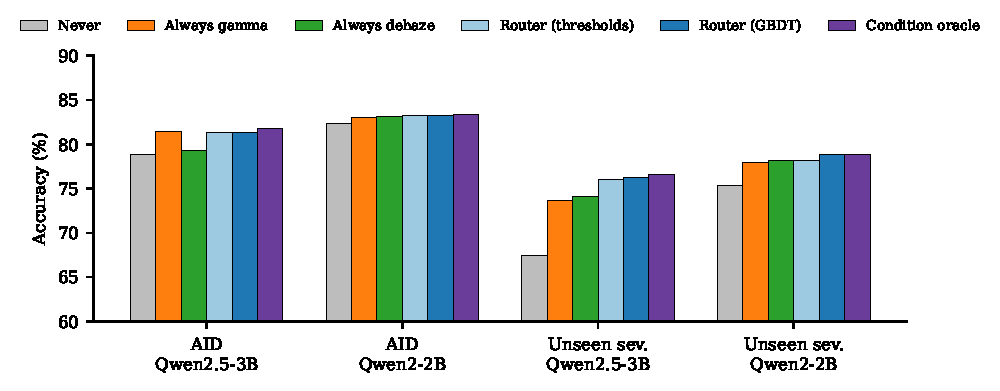
\includegraphics[width=0.85\textwidth]{graphs/transfer_accuracy}
\caption{Accuracy on the transfer sets with the router fitted on UC Merced and applied without change. AID uses severities 1--3; the unseen-severity set uses level 4 only, which is never seen when the router is built. The condition oracle uses the true degradation and the target data's own best operator.}
\label{fig:transfer}
\end{figure*}

\begin{table*}[t]
\centering
\footnotesize
\caption{Transfer results (\%). The detector, the thresholds, and the lookup table are fitted on the UC Merced main study and applied without change. Gains and differences use image-level paired bootstrap 95\% confidence intervals.}
\label{tab:transfer}
\renewcommand{\arraystretch}{1.05}
\setlength{\tabcolsep}{3pt}
\begin{tabular}{|l|c|c|c|c|c|c|c|c|}
\hline
 & \multicolumn{4}{c|}{\textbf{AID (severity 1--3)}} & \multicolumn{4}{c|}{\textbf{Unseen severity (level 4)}} \\
\hline
 & \multicolumn{2}{c|}{\textbf{Qwen2.5-VL-3B}} & \multicolumn{2}{c|}{\textbf{Qwen2-VL-2B}} & \multicolumn{2}{c|}{\textbf{Qwen2.5-VL-3B}} & \multicolumn{2}{c|}{\textbf{Qwen2-VL-2B}} \\
\hline
\textbf{Policy} & \textbf{Acc.} & \textbf{Gain [95\% CI]} & \textbf{Acc.} & \textbf{Gain [95\% CI]} & \textbf{Acc.} & \textbf{Gain [95\% CI]} & \textbf{Acc.} & \textbf{Gain [95\% CI]} \\
\hline
Never enhance & 78.8 & -- & 82.4 & -- & 67.4 & -- & 75.3 & -- \\
Always CLAHE & 80.3 & +1.5 [+0.5, +2.4] & 82.3 & $-$0.1 [$-$0.8, +0.7] & 71.2 & +3.8 [+2.1, +5.6] & 75.5 & +0.2 [$-$1.2, +1.7] \\
Always gamma & \textbf{81.4} & +2.6 [+1.7, +3.6] & 83.0 & +0.6 [$-$0.1, +1.4] & 73.7 & +6.3 [+4.5, +7.9] & 77.9 & +2.6 [+1.1, +4.2] \\
Always dehaze & 79.3 & +0.5 [$-$0.2, +1.3] & 83.1 & +0.8 [+0.0, +1.5] & 74.1 & +6.7 [+5.3, +8.1] & 78.2 & +2.9 [+1.9, +4.0] \\
\hline
\textbf{Router, GBDT detector} & 81.3 & \textbf{+2.5 [+1.6, +3.5]} & \textbf{83.3} & \textbf{+0.9 [+0.1, +1.7]} & \textbf{76.3} & \textbf{+8.9 [+7.0, +10.8]} & \textbf{78.8} & \textbf{+3.6 [+2.0, +5.0]} \\
Router, threshold detector & 81.3 & +2.5 [+1.6, +3.4] & 83.2 & +0.8 [+0.1, +1.6] & 76.0 & +8.6 [+6.6, +10.5] & 78.2 & +2.9 [+1.4, +4.5] \\
\hline
Condition oracle (target table) & 81.8 & +3.0 [+2.1, +3.9] & 83.4 & +1.1 [+0.3, +1.8] & 76.6 & +9.2 [+7.4, +11.0] & 78.9 & +3.6 [+2.1, +5.1] \\
\hline
Router vs best fixed operator & \multicolumn{2}{c|}{$-$0.1 [$-$0.6, +0.3] (gamma)} & \multicolumn{2}{c|}{+0.1 [$-$0.6, +0.9] (dehaze)} & \multicolumn{2}{c|}{+2.3 [+1.1, +3.4] (dehaze)} & \multicolumn{2}{c|}{+0.6 [$-$0.6, +1.8] (dehaze)} \\
Detector accuracy (GBDT / thresholds) & \multicolumn{4}{c|}{92.7\% / 83.3\%} & \multicolumn{4}{c|}{97.0\% / 89.7\%} \\
\hline
\end{tabular}
\end{table*}

Table~\ref{tab:transfer} and Fig.~\ref{fig:transfer} report the router on data that played no part in building it. On AID, whose images come from a different source, size, and set of scene classes, the detector still identified the degradation for 92.7\% of inputs. Its main error was labelling hazy AID inputs as clean (138 of 1,400). The router raised accuracy from 78.8\% to 81.3\% for Qwen2.5-VL-3B (+2.5, CI [+1.6, +3.5]) and from 82.4\% to 83.3\% for Qwen2-VL-2B (+0.9, CI [+0.1, +1.7]), within 0.5 points of the oracle that uses AID's own best operators. On AID, however, the router did not outperform the best fixed operator: always-gamma reached 81.4\% for Qwen2.5-VL-3B, and the difference to the router was $-$0.1 points (CI [$-$0.6, +0.3]). The best fixed operator also changed with the model (gamma for Qwen2.5-VL-3B, dehazing for Qwen2-VL-2B), so it could only have been chosen after testing on AID. The router reached the same accuracy without that choice.

The unseen-severity test is harder: level 4 has denser, coloured haze and darker, noisier low light than any image used to build the router. Never enhancing fell to 67.4\% for Qwen2.5-VL-3B, and the router raised it to 76.3\% (+8.9, CI [+7.0, +10.8]). Here the router outperformed both fixed operators, always-dehaze by 2.3 points (CI [+1.1, +3.4]) and always-gamma by 2.7 points (CI [+1.6, +3.8]), because the two degradations now need clearly different operators: under level-4 haze, dehazing raised accuracy from 63.2\% to 85.3\%, while gamma correction reached only 77.5\%, and under level-4 low light the opposite held (57.2\% for gamma against 51.8\% for dehazing). The detector classified 97.0\% of level-4 inputs correctly; all hazy and low-light inputs were recognised, and the only errors were clean images labelled as degraded. For Qwen2-VL-2B, the router gained 3.6 points and was 0.6 points above always-dehaze, a difference within the confidence interval.

Two further observations hold across the four transfer settings. On these synthetic sets, the threshold router stayed within 0.6 points of the gradient-boosted router, even though its detection accuracy was 7--10 points lower, which shows that most errors of the simple detector fall on inputs where the operator choice matters little. The real data in Section~\ref{sec:real} qualify this result. Using the Qwen2.5-VL-3B lookup table to serve Qwen2-VL-2B on AID gave 83.3\%, identical to the model's own table, so neither the detector nor the table had to be rebuilt for the other model.

\subsection{Real Hazy and Night-Time Imagery}
\label{sec:real}

\begin{table*}[t]
\centering
\footnotesize
\caption{Results on real degradations (\%). RRSHID accuracy is agreement with the VLM's confident answer on the haze-free twin (184 and 304 questions are kept for the two VLMs); CODrone accuracy is against the box labels. The detector and the lookup table are fitted on the UC Merced main study; the few-shot detector additionally sees 30 labelled RRSHID training pairs. Gains use image-level paired bootstrap 95\% confidence intervals.}
\label{tab:real}
\renewcommand{\arraystretch}{1.05}
\setlength{\tabcolsep}{3pt}
\resizebox{\linewidth}{!}{
\begin{tabular}{|l|c|c|c|c|c|c|c|c|}
\hline
 & \multicolumn{4}{c|}{\textbf{RRSHID, real haze (satellite)}} & \multicolumn{4}{c|}{\textbf{CODrone, real night and day (UAV)}} \\
\hline
 & \multicolumn{2}{c|}{\textbf{Qwen2.5-VL-3B}} & \multicolumn{2}{c|}{\textbf{Qwen2-VL-2B}} & \multicolumn{2}{c|}{\textbf{Qwen2.5-VL-3B}} & \multicolumn{2}{c|}{\textbf{Qwen2-VL-2B}} \\
\hline
\textbf{Policy} & \textbf{Acc.} & \textbf{Gain [95\% CI]} & \textbf{Acc.} & \textbf{Gain [95\% CI]} & \textbf{Acc.} & \textbf{Gain [95\% CI]} & \textbf{Acc.} & \textbf{Gain [95\% CI]} \\
\hline
Never enhance & 85.9 & -- & 84.0 & -- & \textbf{70.0} & -- & 69.7 & -- \\
Always CLAHE & 87.0 & +1.1 [$-$3.0, +5.5] & 85.0 & +1.0 [$-$0.9, +3.0] & 69.1 & $-$0.9 [$-$2.5, +0.6] & \textbf{71.4} & +1.7 [+0.4, +3.0] \\
Always gamma & 84.0 & $-$1.9 [$-$5.2, +1.6] & 85.9 & +1.8 [+0.3, +3.4] & 69.2 & $-$0.8 [$-$2.4, +0.7] & 71.2 & +1.5 [+0.1, +2.9] \\
Always dehaze & \textbf{91.8} & +6.0 [+2.2, +9.8] & 89.5 & +5.4 [+2.6, +8.1] & 68.4 & $-$1.6 [$-$3.1, $-$0.2] & 70.3 & +0.6 [$-$0.5, +1.7] \\
\hline
Router, GBDT detector (zero-shot) & 86.1 & +0.3 [$-$3.5, +4.2] & 88.8 & +4.8 [+2.9, +6.9] & 69.2 & $-$0.8 [$-$2.4, +0.7] & 69.7 & 0.0 \\
Router, threshold detector (zero-shot) & 86.7 & +0.8 [$-$3.4, +5.0] & 89.1 & +5.1 [+2.8, +7.5] & 69.2 & $-$0.8 [$-$2.4, +0.7] & 70.9 & +1.2 [0.0, +2.4] \\
\textbf{Router, GBDT detector (few-shot, 30 pairs)} & 89.1 & +3.3 [$-$1.1, +7.6] & \textbf{90.0} & \textbf{+5.9 [+3.3, +8.4]} & -- & -- & -- & -- \\
\hline
Condition oracle (target table) & 92.1 & +6.3 [+2.7, +9.9] & 90.0 & +5.9 [+3.3, +8.4] & 70.0 & 0.0 & 71.4 & +1.7 [+0.4, +3.0] \\
\hline
Degraded inputs only: never / best operator & \multicolumn{2}{c|}{71.7 / 84.2 (dehaze)} & \multicolumn{2}{c|}{68.1 / 79.9 (dehaze)} & \multicolumn{2}{c|}{72.2 / 72.2 (none)} & \multicolumn{2}{c|}{72.0 / 74.0 (gamma, CLAHE)} \\
Degraded inputs only: router zero-shot / few-shot & \multicolumn{2}{c|}{77.7 / 84.2} & \multicolumn{2}{c|}{77.6 / 79.9} & \multicolumn{2}{c|}{70.8 / --} & \multicolumn{2}{c|}{72.0 / --} \\
Detector accuracy: GBDT zero-shot / few-shot / thresholds & \multicolumn{2}{c|}{74.5 / 98.4 / 48.1} & \multicolumn{2}{c|}{77.1 / 99.2 / 46.9} & \multicolumn{4}{c|}{41.2 / -- / 98.4} \\
\hline
\end{tabular}}
\end{table*}

\begin{figure*}[t]
\centering
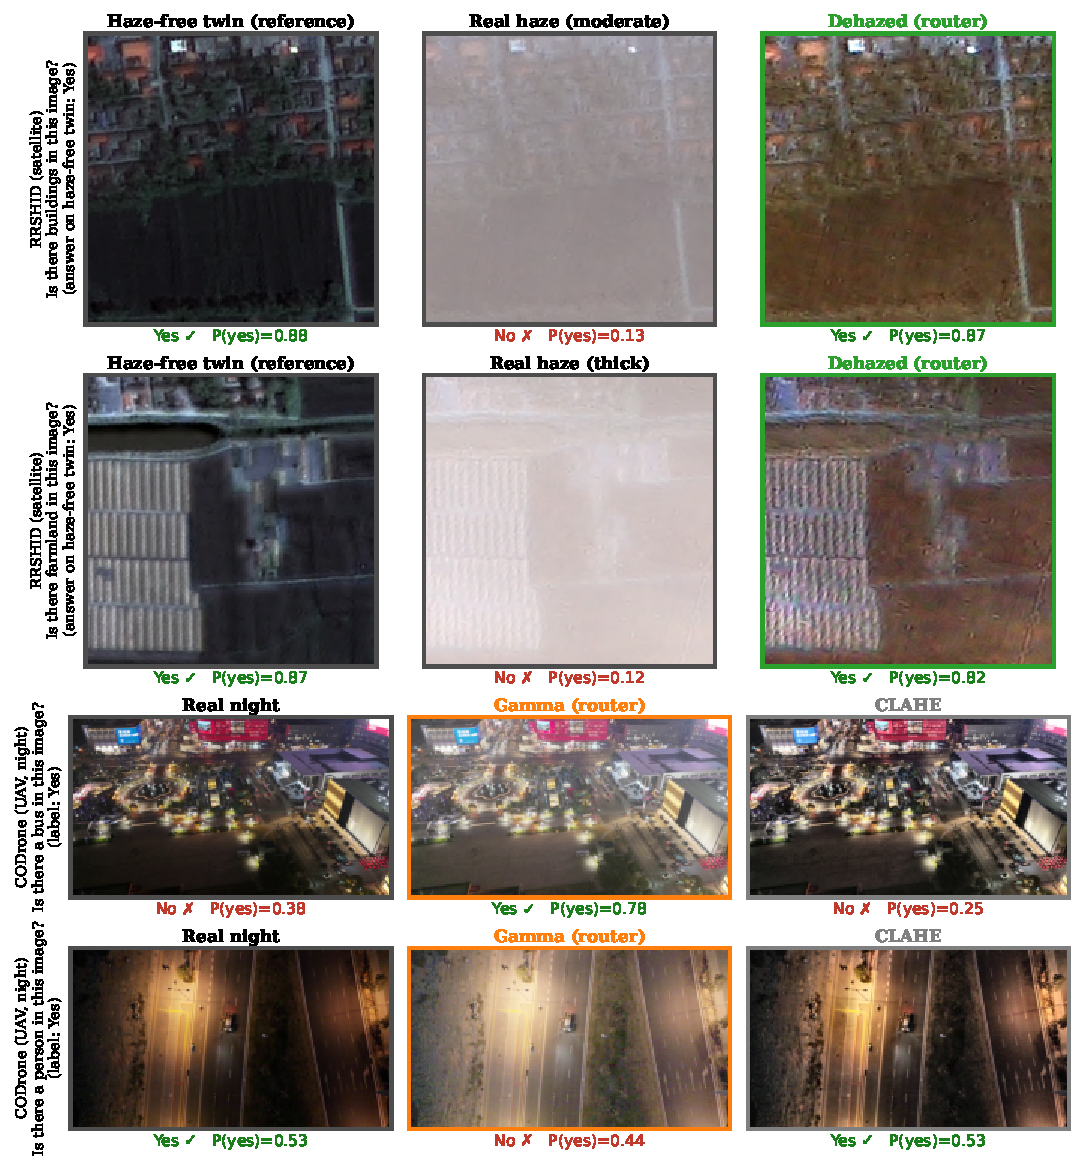
\includegraphics[width=0.8\textwidth]{graphs/real_examples.pdf}
\caption{Real degradations, shown exactly as Qwen2.5-VL-3B received them, with its answers. Top two rows: RRSHID haze-free twin, real hazy input, and the dehazed input selected by the router with the few-shot detector; the reference answer is the model's answer on the haze-free twin. Bottom two rows: CODrone night images, the gamma-corrected input selected by the router, and CLAHE for comparison; the reference is the box label. The rows were chosen to show one success on each dataset and one failure on night imagery; they are not a random sample.}
\label{fig:real}
\end{figure*}

Table~\ref{tab:real} and Fig.~\ref{fig:real} report the router on real degradations. On RRSHID, dehazing remained the right operator for real haze: on hazy inputs it raised agreement with the haze-free answer from 71.7\% to 84.2\% for Qwen2.5-VL-3B and from 68.1\% to 79.9\% for Qwen2-VL-2B, and always dehazing gave the largest overall gain among the fixed operators for both models. The detector built on synthetic haze, however, recognised only 74.5\% and 77.1\% of the RRSHID inputs; its errors were real hazy images labelled as clean, mostly in the thin-haze subset, which then received gamma correction instead of dehazing. The zero-shot router therefore gained 4.8 points for Qwen2-VL-2B but only 0.3 points for Qwen2.5-VL-3B.

The detector is the only part of the router that had to be adapted. Adding the image statistics of 10 labelled pairs per density (30 pairs) from the RRSHID training split raised detection to 98.4\% and 99.2\%, with no real hazy test image labelled clean, and 30 pairs per density gave the same result. With this detector, the router reached the oracle on hazy inputs for both VLMs (84.2\% and 79.9\%). For Qwen2-VL-2B, it matched the oracle overall (90.0\%, +5.9 points, CI [+3.3, +8.4]) and was 0.5 points above always dehazing (CI [0.0, +1.1]). For Qwen2.5-VL-3B, it remained 2.7 points below always dehazing (CI [$-$4.3, $-$1.3]); the whole difference lies on the haze-free images, where the Qwen2.5-VL-3B table applies gamma correction (94.0\% against 99.5\%). Part of this cost comes from the metric, since the reference answer is defined on the haze-free image without enhancement, so any change to that image can only lower agreement. The threshold detector did not benefit from the extra pairs (48\% to 50\%): two statistics cannot separate the dark haze-free RRSHID images (mean luminance 0.22, so most were labelled low light) from real haze.

The CODrone night images behaved differently from the synthetic low light. With a blank image, both VLMs answered \emph{no} to every question (52.8\%), so the 70\% reached with the real images rests on visual evidence. Their mean luminance (0.17) lies close to synthetic severity~1, but their noise estimate is less than half that of the synthetic low-light images, and many contain bright street lights. The gradient-boosted detector, which relies on all 11 statistics, labelled 588 of the 600 night inputs as clean (41.2\% detection overall), whereas the two-threshold detector, which uses luminance alone for low light, recognised 98.4\%. The choice of detector mattered little, because no operator helped much. For Qwen2.5-VL-3B, every operator lowered accuracy on night images (72.2\% without enhancement, 70.8\% with gamma correction); gamma correction corrected 22 night answers and broke 30. For Qwen2-VL-2B, gamma correction and CLAHE raised night accuracy from 72.0\% to 74.0\%, and the threshold router gained 1.2 points (CI [0.0, +2.4]), the same as the oracle with the source table. The night images in CODrone are lit urban scenes captured by a modern camera, not the uniformly dark and noisy inputs simulated here, and both VLMs answered them at least as accurately as the daytime images of the same set (72.2\% and 72.0\% at night against 66.8\% and 66.2\% by day).

\subsection{Why Enhancement Hurts: Evidence Drift}

When an operator turned a correct answer wrong, it had changed the image more. For Qwen2.5-VL-3B, the mean CIELAB colour difference between the input and the enhanced image was 37.8 for harmful enhancements against 34.1 for harmless ones, and the high-frequency energy ratio was 2.00 against 1.91; Qwen2-VL-2B gave nearly the same values (37.6 against 34.1, and 2.11 against 1.91). The mean hue shift did not differ for Qwen2.5-VL-3B (3.48 against 3.50), so harmful changes act mainly through lightness and contrast. The effect is modest on average, which explains why the per-sample gate could not exploit these measures reliably, but it is consistent with the higher sensitivity of colour- and texture-dependent questions.

\subsection{Computational Cost}

The router adds little cost to inference. On a 2-vCPU Intel Xeon instance at 2.1\,GHz, computing the 11 statistics took 3.5\,ms per 256$\times$256 image and 14.0\,ms per 512$\times$512 image, the classifier prediction about 3.6\,ms, and the selected operator at most 8.3\,ms and 10.4\,ms (dark-channel dehazing; CLAHE 0.9 and 3.0\,ms, gamma 0.5 and 2.3\,ms), for at most about 15\,ms and 28\,ms per image in total. The threshold detector removes the classifier and reads only two of the statistics. A single VLM answer took 0.4--2.2\,s on a T4 GPU in our setting, depending on the model and image size, so routing adds a few percent to the end-to-end latency and requires no GPU memory. By contrast, methods that place a multimodal model in the restoration loop~\cite{cai2025degradationaware, huang2026docintent, zeng2026fixbeforesearch} require at least one additional model pass per input.

\begin{table*}[t]
\footnotesize
\setlength{\tabcolsep}{3pt}
\caption{Comparison with representative methods that address degraded or suboptimal inputs to vision and vision-language models.}
\centering
\resizebox{\linewidth}{!}{
\begin{tabular}{|l|l|l|c|c|l|}
\hline
\textbf{Method} & \textbf{Domain} & \textbf{What is adapted per input} & \textbf{Trains a model?} & \textbf{Extra model calls?} & \textbf{Judged by} \\
\hline
REOBench~\cite{li2025reobench} & Earth observation & -- (benchmark) & No & -- & Task accuracy under 12 corruptions \\
RemoteShield~\cite{min2026remoteshield} & Earth observation & -- (robust training) & Yes (the MLLM) & No & Task accuracy on clean and perturbed inputs \\
Plug-and-play detector~\cite{wu2024plugplay} & Aerial detection & Enhancement and fusion branch & Yes (the branch) & No & Detection accuracy in haze \\
DA-CLIP~\cite{luo2024daclip} & Natural images & Restoration conditioning & Yes (controller and restorer) & No & Restored image quality \\
Cai et al.~\cite{cai2025degradationaware} & Natural images & Restoration model & No (VLM used zero-shot) & Yes (VLM classifier) & Restored image quality \\
VQ-TTT~\cite{xing2025vqparadox} & Natural images & Input kernel and vision-encoder LoRA & Yes (test-time tuning) & No & MLLM benchmark accuracy \\
CARES~\cite{kimhi2025cares} & Documents, natural images & Input resolution & Yes (selector) & No & VLM accuracy and compute \\
DocIntent~\cite{huang2026docintent} & Document VQA & Restoration tool & No & Yes & Answer accuracy \\
V-QPP-Bench~\cite{zeng2026fixbeforesearch} & Multimodal RAG & Preprocessing tool & Optional & Yes & Retrieval and answer accuracy \\
\hline
\textbf{Router (ours)} & \textbf{Remote sensing} & \textbf{Enhancement operator} & \textbf{Small classifier; VLM frozen} & \textbf{No} & \textbf{Answer accuracy of the frozen VLM} \\
\hline
\end{tabular}
}
\label{tab:Model_Comparison}
\end{table*}

\subsection{Comparison with Prior Work}

Table~\ref{tab:Model_Comparison} places the router beside representative methods. A direct accuracy comparison is not possible because these methods address different tasks, datasets, and models, so the table compares what each method adapts, what it costs, and how it is judged. The idea of detecting a degradation and then applying a matching restoration is not new: DA-CLIP~\cite{luo2024daclip} and Cai~et~al.~\cite{cai2025degradationaware} follow it for natural images, and plug-and-play enhancement has been used for aerial detection in haze~\cite{wu2024plugplay}. These methods use learned restorers and are judged by image quality or detection accuracy. The present work keeps the restoration classical and asks a different question: whether degradation-aware selection improves the answers of a frozen remote-sensing VLM, whether it beats simply enhancing every image, and whether the selector survives a change of dataset, model, and severity. VQ-TTT~\cite{xing2025vqparadox} and CARES~\cite{kimhi2025cares} adapt the input per image for multimodal models but train a module and do not select an enhancement operator, and DocIntent~\cite{huang2026docintent} and V-QPP-Bench~\cite{zeng2026fixbeforesearch} place the multimodal model in the loop. V-QPP-Bench reports that off-the-shelf models select tools poorly; our results complement this finding, since for synthetic haze and low light a detector on image statistics selects the operator well enough to match an oracle that knows the true degradation, without any call to the VLM, and for real haze it does so after seeing 30 labelled real pairs.

\subsection{Deployment Guidelines}

The results support four recommendations. \textbf{Do not enhance by default}: on clean images, CLAHE cost about 3 points for both VLMs, for Qwen2-VL-2B always applying CLAHE lowered overall accuracy, and on real night images every operator lowered the accuracy of Qwen2.5-VL-3B. \textbf{Detect the degradation first, and check the detector on real data}: on synthetic data even two thresholds were enough for routing, but on real haze a detector built from synthetic haze missed thin haze, and on real night images the full detector missed almost everything that the luminance threshold caught. A few labelled real images per degradation fixed the haze detector without touching the VLM. \textbf{Expect the largest benefit when degradations are strong}: on mild AID degradations, always applying the right single operator was as good as routing, but which operator was right depended on the model, and under the unseen level-4 degradations and real haze the gap between operators was large. \textbf{Check image dependence before evaluating preprocessing}: a blank-image control costs one extra run per question and shows whether a benchmark can measure visual effects at all.


\section{Conclusion}

This study examined whether classical enhancement helps frozen VLMs answer questions about degraded remote-sensing images, and proposed a lightweight router that selects the enhancement per image without fine-tuning or querying the VLM. Two frozen models, Qwen2.5-VL-3B and Qwen2-VL-2B, answered 2,100 scene, surface, and object questions on 700 UC Merced images under clean, hazy, and low-light conditions at three severities, with four enhancement operators and a blank-image control, giving 27,300 scored runs per model. Answers were read from first-token probabilities, so the full study ran on two free-tier T4 GPUs.

The central finding is that blind enhancement is not a safe default. CLAHE lowered clean-image accuracy by about 3 points for both models, dehazing did not help low-light inputs, and each degradation had its own best operator: dehazing for haze and gamma correction for low light. A router that classifies the degradation from 11 global statistics and looks up its best operator raised overall accuracy from 79.6\% to 83.3\% for Qwen2.5-VL-3B and from 85.2\% to 86.2\% for Qwen2-VL-2B, matched an oracle that knows the true degradation, and outperformed the best fixed operator for both models. Its benefit grew with severity, reaching 10.6 points under strong haze for Qwen2.5-VL-3B, at 15--28\,ms of CPU time per image and with no VLM calls. A two-threshold detector gave the same accuracy, so the benefit comes from routing by degradation type rather than from the classifier.

Fitted once on UC Merced and applied unchanged, the router kept its gain on AID (+2.5 and +0.9 points) and on an unseen, stronger degradation level (+8.9 and +3.6 points), and the lookup table transferred between the two VLMs without loss. On mild AID degradations, a single fixed operator chosen in hindsight was as accurate as the router, but the right operator differed between the two models; under the unseen level, the router outperformed every fixed operator for Qwen2.5-VL-3B.

Real degradations showed where the router holds and where it needs care. On real hazy satellite images, dehazing remained the right operator, raising agreement with the haze-free answer by about 12 points on hazy inputs, but a detector built only on synthetic haze missed part of the real haze, mostly thin haze. Adding 30 labelled real image pairs to the detector, with the VLM and the lookup table unchanged, raised detection to 98--99\% and brought the router to oracle accuracy on hazy inputs. On real night-time UAV images, which were lit rather than uniformly dark, no operator changed accuracy by more than 2 points, and the full detector failed where a luminance threshold succeeded.

Several directions follow from this work. The study used small general-purpose VLMs; larger and remote-sensing-specific models such as GeoChat~\cite{kuckreja2024geochat} may respond differently to enhancement. The action set was small and classical; learned restoration networks could widen the gap between the best and worst operators and make routing more valuable. The detector should be trained on real as well as synthetic degradations, since the night results showed that synthetic noise statistics do not describe real night imagery. A single operator per condition cannot serve all severities, as the mild low-light case for Qwen2-VL-2B showed, so severity-aware tables are a natural extension. Finally, mixed degradations, such as haze combined with low light, call for routing over sequences of operators rather than a single choice.


\bibliographystyle{IEEEtran}
\bibliography{references}

\vspace{11pt}

\begin{IEEEbiographynophoto}{Syed Muhammad Hamza Tauqeer}
received the B.S. degree in Electronics Engineering from the University of Engineering \& Technology, Taxila, Pakistan, in 2022, and the M.S. degree in Electrical Engineering with a specialization in AI \& Autonomous Systems from the Military College of Signals, National University of Sciences and Technology (NUST), Pakistan, in 2026. His research interests include machine learning, computer vision, remote sensing, vision-language models, degradation-aware image enhancement, and data-driven modeling of renewable energy systems.
\end{IEEEbiographynophoto}

\begin{IEEEbiographynophoto}{Muhammad Talha} received his B.E. degree in Electrical Engineering from the School of Electrical Engineering and Computer Science (SEECS), National University of Sciences and Technology (NUST), Pakistan. His research interests revolve around deep learning, with a focus on building and training models for various data-driven applications.
\end{IEEEbiographynophoto}

\begin{IEEEbiographynophoto}{Huma Ghafoor}
received the Ph.D. degree in electrical engineering from the University of Ulsan, South Korea, in 2018. She began working as a Postdoctoral Researcher after her Ph.D. at the Networked Systems Laboratory, Inha University, Incheon, and held the position until January 2019. She is currently an Associate Professor with the School of Electrical Engineering and Computer Science, NUST. Her research interests include vehicular networks, maritime networks, underwater networks, with a focus on networking protocols.
\end{IEEEbiographynophoto}

\begin{IEEEbiographynophoto}{SEUNG YEOB NAM}(Senior Member, IEEE) received the B.S., M.S., and Ph.D. degrees in electrical engineering from Korea Advanced Institute of Science and Technology (KAIST), Daejeon, South Korea, in 1997, 1999, and 2004, respectively. From 2004 to 2006, he was a postdoctoral Research Fellow with the CyLab, Carnegie Mellon University. In 2007, he joined the Department of Information and Communication Engineering, Yeungnam University, Gyeongsan, South Korea, where he is currently a Professor. From January 2012 to January 2013, he was a Visiting Professor with the Department of Electrical and Computer Engineering, Carnegie Mellon University. His research interests include network security, blockchain, network management, and wireless networks. He received the 2022 Best Paper Award from Digital Communications and Networks (DCN).
\end{IEEEbiographynophoto}

\vfill

\end{document}
